\documentclass[12pt,a4paper]{article}
\usepackage[margin=2cm]{geometry}
\usepackage{xeCJK}
\usepackage{fontspec}
\setCJKmainfont{Noto Serif CJK TC}[Script=CJK]
\usepackage{amsmath,amssymb}
\usepackage{graphicx}
\usepackage{fancyhdr}
\setlength{\headheight}{14.5pt}
\addtolength{\topmargin}{-2.5pt}
\usepackage{hyperref}
\usepackage{listings}
\usepackage{enumitem}
\usepackage{titlesec}
\usepackage{caption}
\usepackage{indentfirst}
\usepackage{float}
\usepackage{forest}
\setlength{\parindent}{2em}
\pagestyle{fancy}
\fancyhf{}
\cfoot{\thepage}
\linespread{1.3}

\usepackage{multirow}
\usepackage{booktabs}   % 放在 preamble
\usepackage{graphicx}


% tikz tools for ER diagram
\usepackage{tikz}
\usetikzlibrary{shapes,positioning,calc}
\colorlet{lightgray}{gray!20}


\usepackage{minted}
\setminted{
    linenos,                % 行號
    frame=lines,            % 上下框線
    framesep=5pt,           % 程式碼與邊框距離
    numbersep=8pt,          % 行號與程式碼距離
    fontsize=\scriptsize,   % 字體大小
    breaklines,             % 自動換行
    tabsize=4,              % tab 寬度
    rulecolor=\color{black},% 框線顏色
    xleftmargin=1.5em       % 左側縮排
}


\title{資料庫管理 HW02}
\author{B12508026戴偉璿}
\date{}

\begin{document}

\maketitle

\lhead{資料庫管理 HW02}
\rhead{B12508026戴偉璿}

\begin{enumerate}
    \item
    \begin{enumerate}
        \item
        \begin{enumerate}
            \item \textbf{TRUE}, because \texttt{DEAN} is a \textbf{relation} between \texttt{COLLEGE} and \texttt{INSTRUCTOR}; and \texttt{CHAIR} is a \textbf{relation} between \texttt{DEPT} and \texttt{INSTRUCTOR}.
            \item \textbf{FALSE}, there's no further restriction on \texttt{DEAN} and \texttt{CHAIR}, so one \texttt{INSTRUCTOR} can be a \texttt{CHAIR} and a \texttt{DEAN} at the same time.
            \item \textbf{TRUE}, the relation between \texttt{STUDENT} and \texttt{HAS} is a \textbf{(0, 1)} relation, so one \texttt{STUDENT} can \texttt{HAS} zero or one \texttt{DEPT}.
            \item \textbf{TRUE}, the cardinality between \texttt{STUDENT} and \texttt{TAKES} is \textbf{(0, N)}, so one student may take zero or more sections; while the cardinality between \texttt{SECTION} and \texttt{TAKES} is \textbf{(5, N)}, so one section must be taken by five or more students.
            \item \textbf{TRUE}, the cardinality between \texttt{COURSE} and \texttt{SECTION} is \textbf{(1, 1)}, so one section must be related to exactly one course.
        \end{enumerate}
        \item As the following diagram:
        
        \begin{figure}[H]
            \centering
            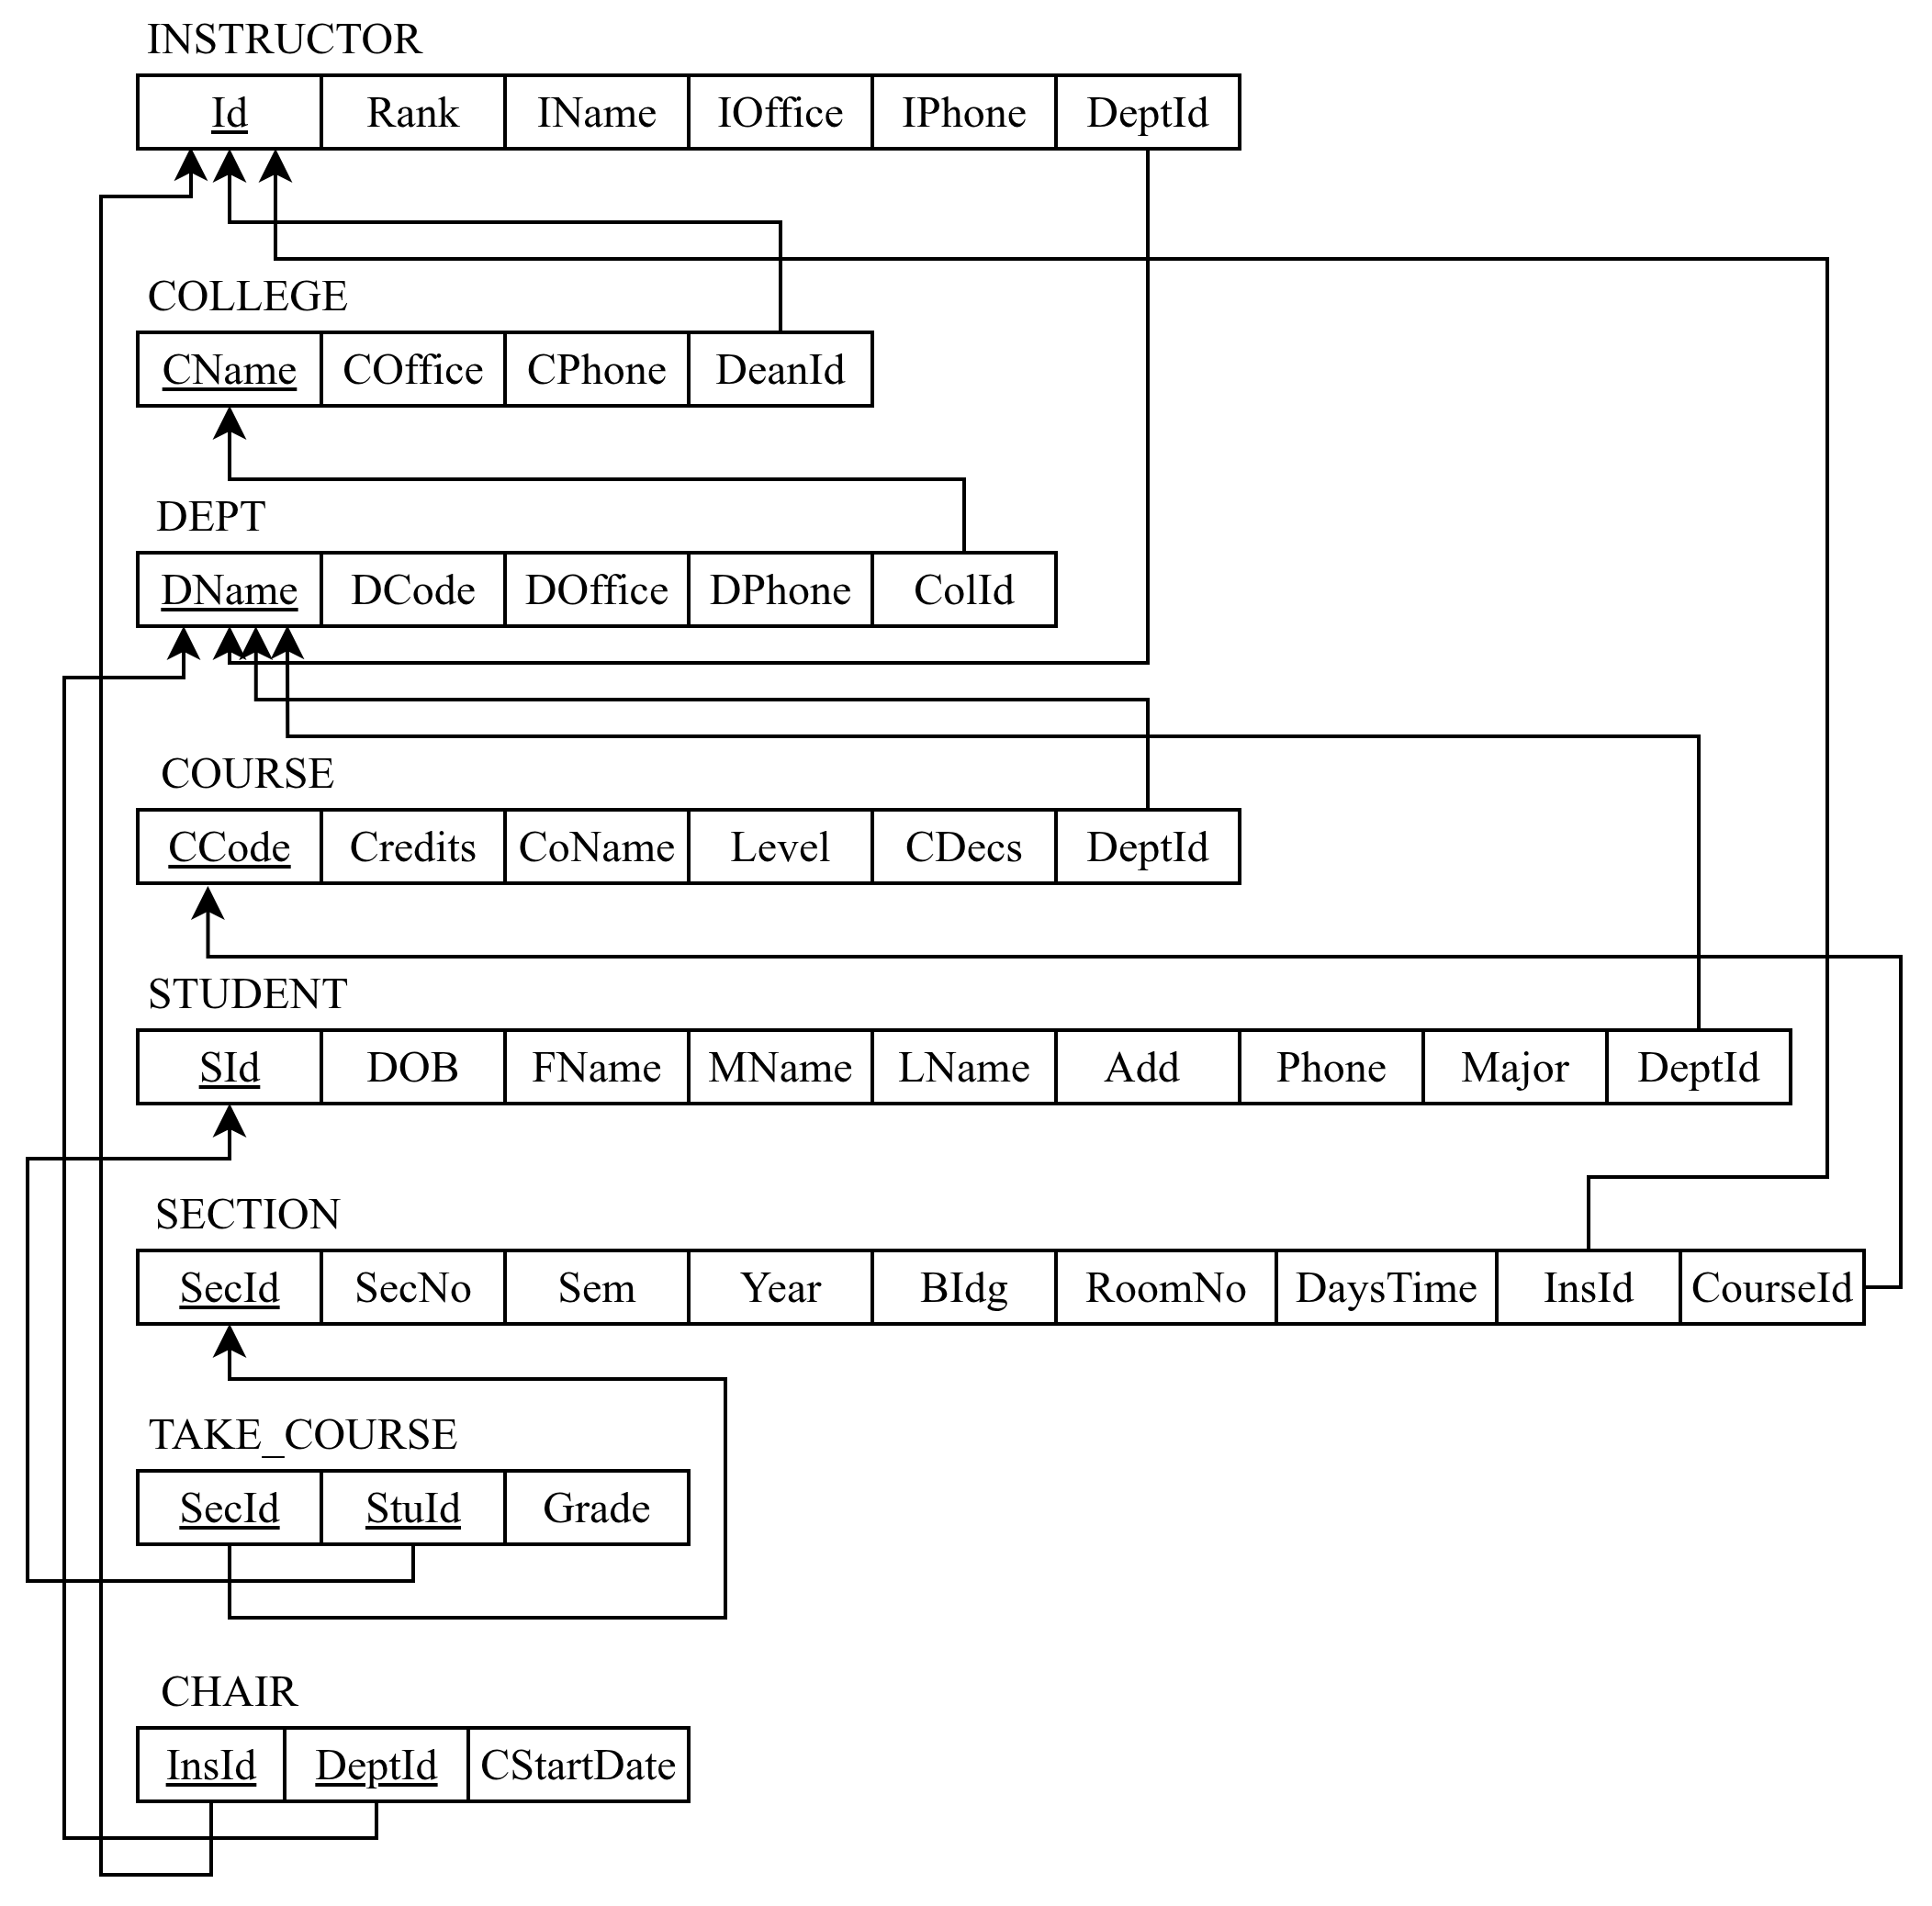
\includegraphics[width=0.6\textwidth]{src/1B.png}
            \caption{Relational Schema Diagram}
            \label{fig:ER_diagram}
        \end{figure}

    \end{enumerate}
    \item \begin{enumerate}
        \item To record the full history of students' take or drop sections, we can just add more attributes to the \texttt{TAKES} relation. But it may cause some problems while querying the final result and grade (user must find the last record of the log to reach). So I decide to create a new weak entity to record the operation log.\\
        If the operation is add, the \texttt{drop\_data} would be record as NULL; vice versa.\\
        \begin{figure}[H]
            \centering
            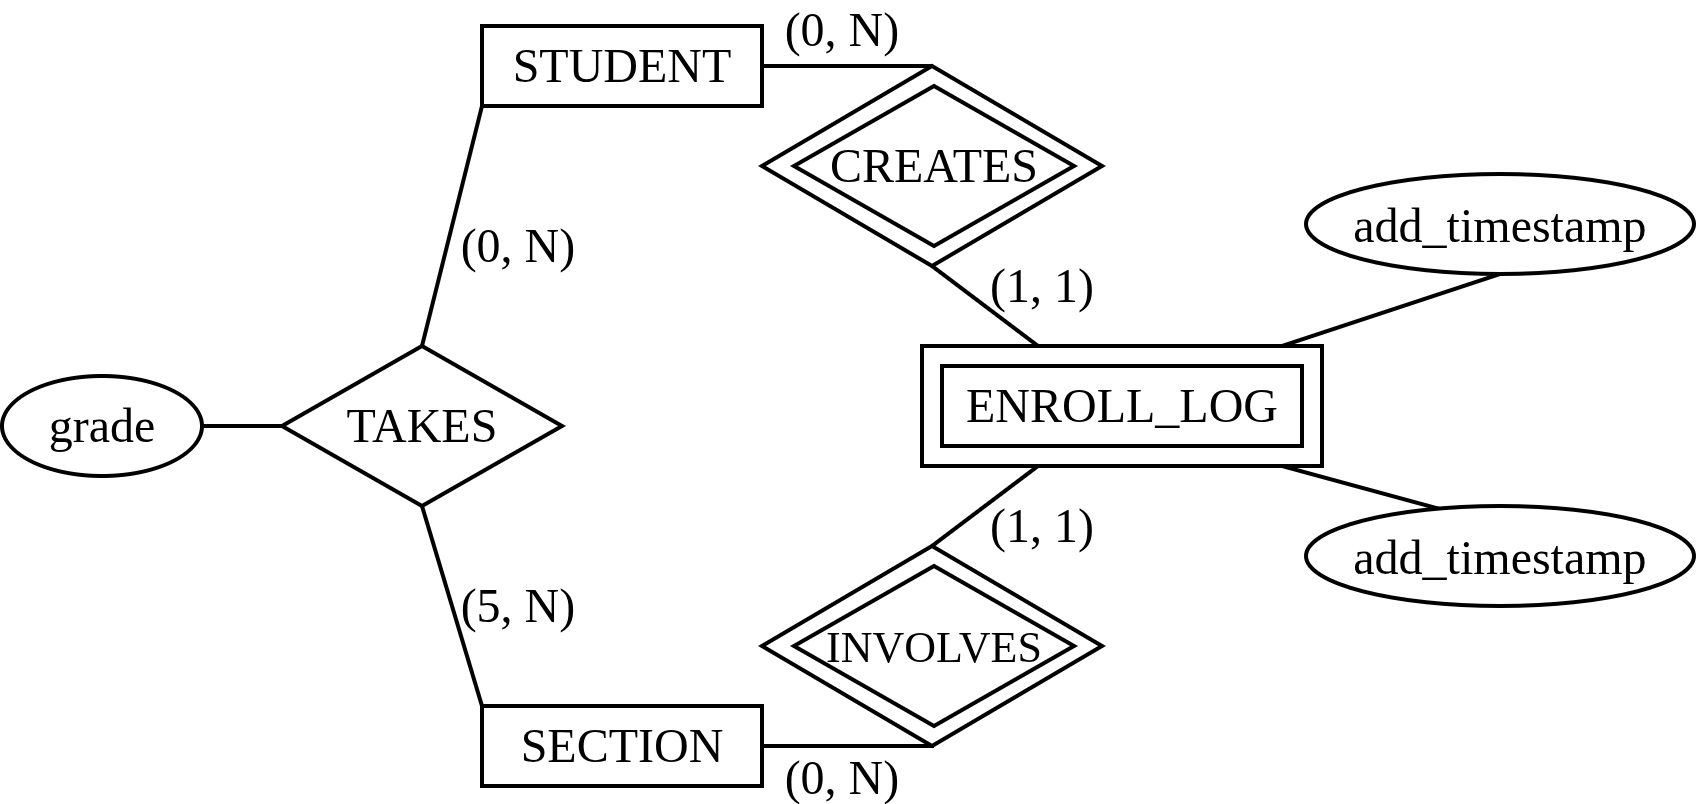
\includegraphics[width=0.6\textwidth]{src/2A.png}
            \caption{ER Diagram with Operation Log}
            \label{fig:ER_diagram_with_log}
        \end{figure}
        \item As the following diagram:
        \begin{figure}[H]
            \centering
            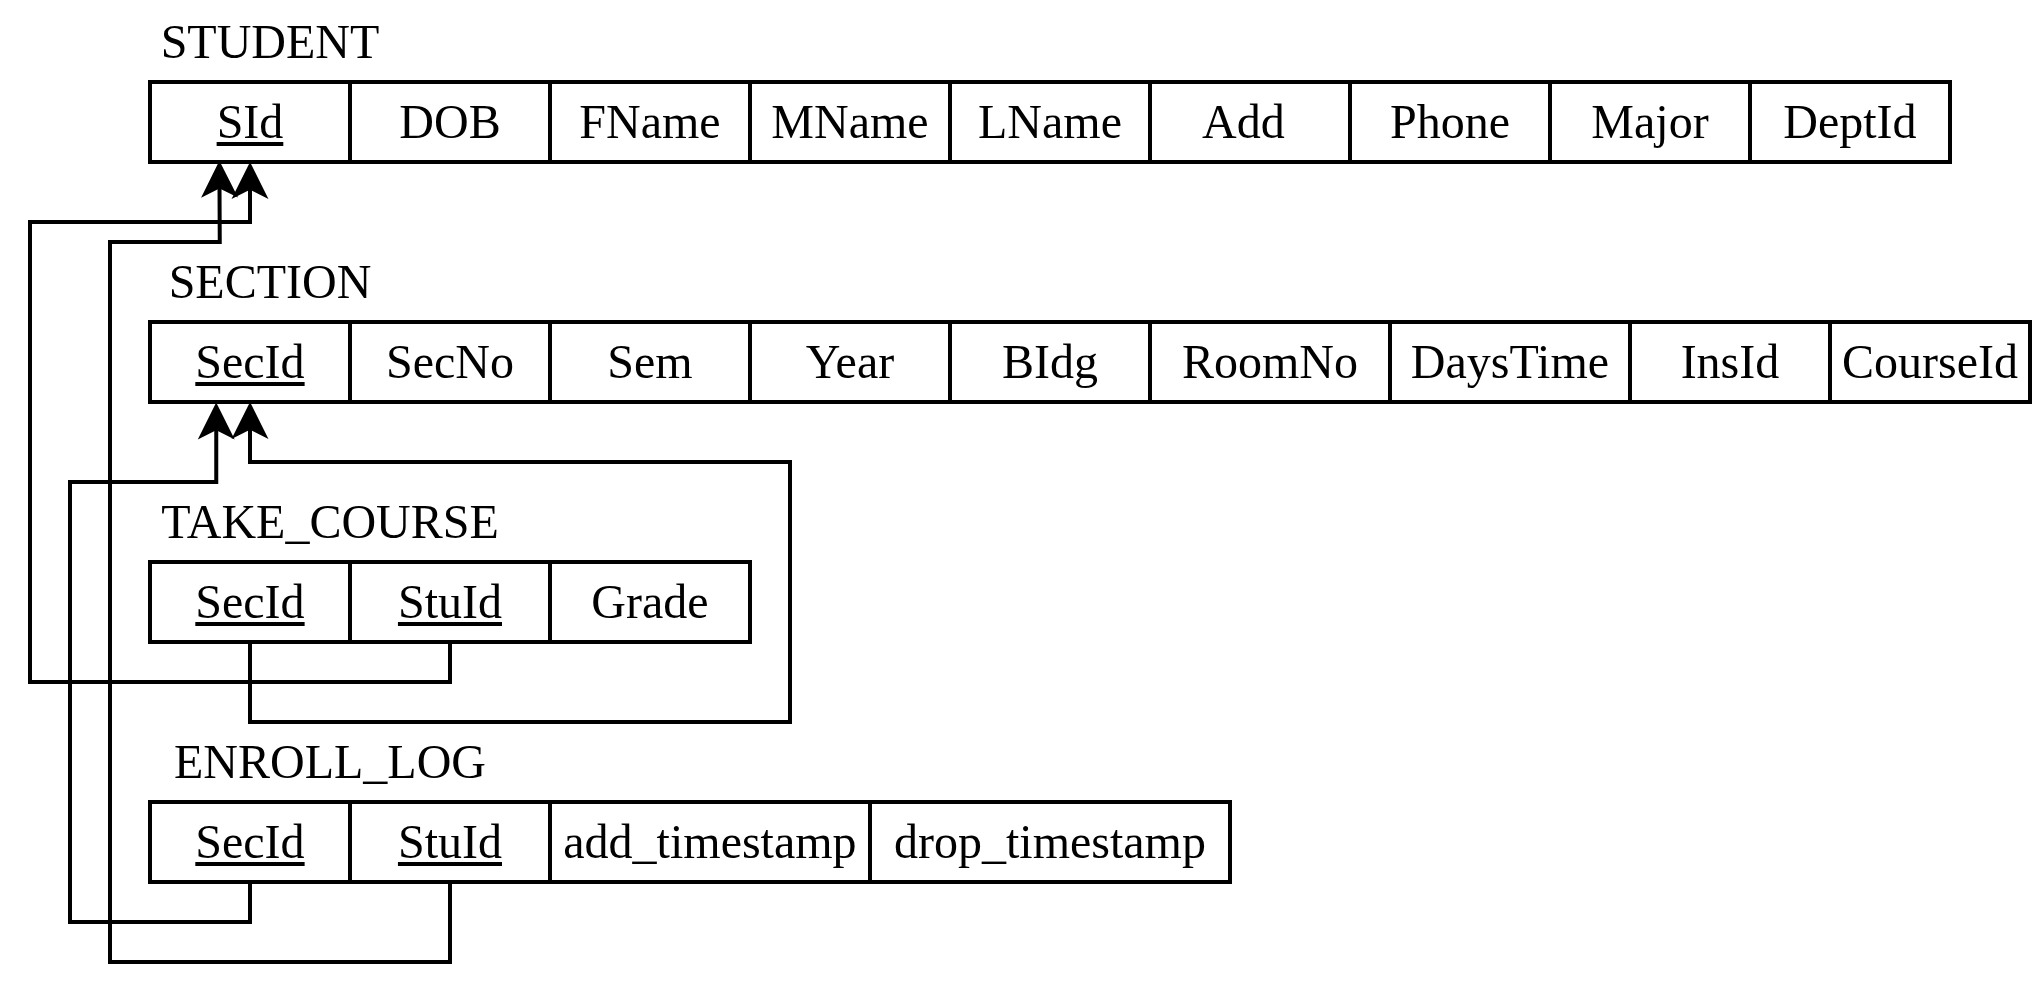
\includegraphics[width=0.6\textwidth]{src/2B.png}
            \caption{Relational Schema Diagram with Advisor}
            \label{fig:ER_diagram_with_advisor}
        \end{figure}
    \end{enumerate}
    \item 
    \begin{enumerate}
        \item
        \begin{minted}{sql}
        SELECT br.Card_no, br.Name, COUNT(*) AS LoanRec
        FROM BOOK_LOANS bl
        JOIN BORROWER br ON bl.Card_no = br.Card_no
        WHERE bl.Branch_id = '[ASSIGNED_BRANCH_ID]'
        GROUP BY br.Card_no, br.Name
        ORDER BY LoanRec DESC;
        \end{minted}
        \item
        \begin{minted}{sql}
        SELECT lib.Branch_id, lib.Branch_name, COUNT(*) AS LoanRec
        FROM BOOK_LOANS bl
        JOIN LIBRARY_BRANCH lib ON lib.Branch_id = bl.Branch_id
        WHERE bl.Date_out BETWEEN '2024-01-01' AND '2024-12-31'
        GROUP BY lib.Branch_id, lib.Branch_name
        ORDER BY LoanRec DESC;
        \end{minted}
        \item
        \begin{minted}{sql}
        SELECT bk.Book_id, bk.Title, COUNT(DISTINCT ba.Author_id) AS AuthorNum, bc.No_of_copies, COUNT(DISTINCT bl.Loan_id) AS LoanRec
        FROM BOOK_LOANS bl
        JOIN BOOK bk ON bl.Book_id = bk.Book_id
        JOIN BOOK_AUTHORS ba ON bl.Book_id = ba.Book_id
        JOIN BOOK_COPIES bc ON bl.BOOK_id = bc.BOOK_id AND bl.Branch_id = bc.Branch_id
        WHERE bl.Branch_id = (
            SELECT bl2.Branch_id
            FROM BOOK_LOANS bl2
            JOIN LIBRARY_BRANCH lib ON lib.Branch_id = bl2.Branch_id
            WHERE bl2.Date_out BETWEEN '2024-01-01' AND '2024-12-31'
            GROUP BY bl2.Branch_id
            ORDER BY COUNT(*) DESC
            LIMIT 1
        )
        AND bl.Date_out BETWEEN '2024-01-01' AND '2024-12-31'
        GROUP BY bk.Book_id, bk.Title, bc.No_of_copies
        ORDER BY LoanRec DESC;
        \end{minted}

        \item
        \begin{minted}{sql}
        SELECT bk.Book_id, bk.Title, lib.Branch_name, bc.No_of_copies
        FROM BOOK bk
        JOIN BOOK_COPIES bc ON bk.Book_id = bc.Book_id
        JOIN LIBRARY_BRANCH lib ON bc.Branch_id = lib.Branch_id
        WHERE bk.Book_id IN (
            SELECT ba.Book_id
            FROM BOOK_AUTHOR ba
            GROUP BY ba.Book_id
            HAVING COUNT(DISTINCT ba.Author_id) = 1
        );
        \end{minted}
        \item
        \begin{minted}{sql}
        --Add new column to the DB
        ALTER TABLE BOOK_LOANS
        ADD COLUMN Date_return DATE;

        --Execute Query
        SELECT bk.Title, lib.Branch_name, bc.No_of_copies - COUNT(bl.Loan_id) AS AvaiCopies
        FROM BOOK bk
        JOIN BOOK_COPIES bc ON bk.Book_id = bc.Book_id
        JOIN LIBRARY_BRANCH lib ON bc.Branch_id = lib.Branch_id
        LEFT JOIN BOOK_LOANS bl ON bk.Book_id = bl.Book_id AND bc.Branch_id = bl.Branch_id AND bl.Date_return IS NULL
        GROUP BY bk.Title, lib.Branch_name, bc.No_of_copies
        \end{minted}
    \end{enumerate}
    \item
    \begin{enumerate}
        \item As the following tables:\\
         BOOK
         \begin{table}[H]
         \centering
         \resizebox{\textwidth}{!}{%
         \begin{tabular}{|l|l|l|p{4cm}|l|}
         \hline
         Column Name & Data Type & Key & Constraint & Domain \\
         \hline
         Book\_id & varchar(15) & PK & Not Null, Unique &  \\
         Title & varchar(100) &  & Not Null &  \\
         Publisher\_name & varchar(50) & FK $\rightarrow$ PUBLISHER(Name) & Not Null &  \\
         \hline
         \end{tabular}}
         \end{table}

         BOOK\_AUTHORS
         \begin{table}[H]
         \centering
         \resizebox{\textwidth}{!}{%
         \begin{tabular}{|l|l|l|p{4cm}|l|}
         \hline
         Column Name & Data Type & Key & Constraint & Domain \\
         \hline
         Book\_id & varchar(15) & PK, FK $\rightarrow$ BOOK(Book\_id) & Not Null &  \\
         Author\_name & varchar(50) & PK & Not Null &  \\
         \hline
         \end{tabular}}
         \end{table}

         PUBLISHER
         \begin{table}[H]
         \centering
         \resizebox{\textwidth}{!}{%
         \begin{tabular}{|l|l|l|p{4cm}|l|}
         \hline
         Column Name & Data Type & Key & Constraint & Domain \\
         \hline
         Name & varchar(50) & PK & Not Null, Unique &  \\
         Address & varchar(100) &  &  &  \\
         Phone & varchar(15) &  &  &  \\
         \hline
         \end{tabular}}
         \end{table}

         BOOK\_COPIES
         \begin{table}[H]
         \centering
         \resizebox{\textwidth}{!}{%
         \begin{tabular}{|l|l|l|p{4cm}|l|}
         \hline
         Column Name & Data Type & Key & Constraint & Domain \\
         \hline
         Book\_id & varchar(15) & PK, FK $\rightarrow$ BOOK(Book\_id) & Not Null &  \\
         Branch\_id & varchar(10) & PK, FK $\rightarrow$ LIBRARY\_BRANCH(Branch\_id) & Not Null &  \\
         No\_of\_copies & int &  & Not Null, CHECK $\geq 0$ & $\{0,1,2,\dots\}$ \\
         \hline
         \end{tabular}}
         \end{table}

         BOOK\_LOANS
         \begin{table}[H]
         \centering
         \resizebox{\textwidth}{!}{%
         \begin{tabular}{|l|l|l|p{4cm}|l|}
         \hline
         Column Name & Data Type & Key & Constraint & Domain \\
         \hline
         Book\_id & varchar(15) & PK, FK $\rightarrow$ BOOK(Book\_id) & Not Null &  \\
         Branch\_id & varchar(10) & PK, FK $\rightarrow$ LIBRARY\_BRANCH(Branch\_id) & Not Null &  \\
         Card\_no & varchar(10) & PK, FK $\rightarrow$ BORROWER(Card\_no) & Not Null &  \\
         Date\_out & date & PK & Not Null &  \\
         Due\_date & date &  & Not Null &  \\
         Date\_return & date &  & 可為 Null &  \\
         \hline
         \end{tabular}}
         \end{table}

         LIBRARY\_BRANCH
         \begin{table}[H]
         \centering
         \resizebox{\textwidth}{!}{%
         \begin{tabular}{|l|l|l|p{4cm}|l|}
         \hline
         Column Name & Data Type & Key & Constraint & Domain \\
         \hline
         Branch\_id & varchar(10) & PK & Not Null, Unique &  \\
         Branch\_name & varchar(50) &  & Not Null &  \\
         Address & varchar(100) &  &  &  \\
         \hline
         \end{tabular}}
         \end{table}

         BORROWER
         \begin{table}[H]
         \centering
         \resizebox{\textwidth}{!}{%
         \begin{tabular}{|l|l|l|p{4cm}|l|}
         \hline
         Column Name & Data Type & Key & Constraint & Domain \\
         \hline
         Card\_no & varchar(10) & PK & Not Null, Unique &  \\
         Name & varchar(50) &  & Not Null &  \\
         Address & varchar(100) &  &  &  \\
         Phone & varchar(15) &  &  &  \\
         \hline
         \end{tabular}}
         \end{table}

    \end{enumerate}
    
\end{enumerate}



\end{document}